\documentclass{article}
\usepackage[MeX]{polski}
\usepackage[utf8]{inputenc}
\usepackage{amsfonts}
\usepackage{amsthm}
\usepackage{fullpage}
\usepackage{graphics}

\title{Rozwiązanie drugiego zadania z~piątej listy z~Mechaniki Kwantowej}
\author{BP PP RW RP}
\date{\today}

\begin{document}

\maketitle

\paragraph{(a)}

Gęstość prawdopodobieństwa znalezienia cząstki w~miejscu $x$ będącej w~stanie $\psi$
zgodnie z~postulatem wyraża się wzorem:
\[
f(x) = |\langle\psi_x|\psi\rangle|^2
\]
gdzie $\psi_x$ jest zewnętrznym wektorem własnym odpowiadającym wartości własnej $x$, tzn.
$\psi_x(y) = \delta(y - x)$.

A zatem:
\begin{eqnarray*}
f_0(x) & = & \left|\int\limits_{-\infty}^\infty \overline{\delta(y - x)}
	\left(\frac{\pi\hbar}{m\omega}\right)^{-\frac{1}{4}}e^{-\frac{m\omega}{2\hbar}y^2}dy
	\right|^2 =
	\left(\frac{\pi\hbar}{m\omega}\right)^{-\frac{1}{2}}e^{-\frac{m\omega}{\hbar}x^2} \\
f_1(x) & = & \left|\int\limits_{-\infty}^\infty \overline{\delta(y - x)}
	\frac{1}{\sqrt{2}}\left(\frac{\pi\hbar}{m\omega}\right)^{-\frac{1}{4}}
	2\sqrt{\frac{m\omega}{\hbar}}ye^{-\frac{m\omega}{2\hbar}y^2}dy\right|^2 =
	\left(\frac{\pi\hbar}{m\omega}\right)^{-\frac{1}{2}}2\frac{m\omega}{\hbar}x^2
	e^{-\frac{m\omega}{\hbar}x^2} \\
f_2(x) & = & \frac{1}{2}\left(\frac{\pi\hbar}{m\omega}\right)^{-\frac{1}{2}}
	\left(2\frac{m\omega}{\hbar}x^2 - 1\right)^2e^{-\frac{m\omega}{\hbar}x^2} \\
\end{eqnarray*}

Przechodząc do bezwymiarowej zmiennej $\xi=\alpha{}x$, 
gdzie $\alpha=\sqrt{\frac{m\omega}{\hbar}}$ otrzymujemy:
\begin{eqnarray*}
f_0(\xi) & = & \frac{1}{\sqrt{\pi}}e^{-\xi^2} \\
f_1(\xi) & = & \frac{2\xi^2}{\sqrt{\pi}}e^{-\xi^2} \\
f_2(\xi) & = & \frac{1}{2\sqrt{\pi}}\left(2\xi^2 - 1\right)^2e^{-\xi^2} \\
\end{eqnarray*}

W~mechanice klasycznej mamy
\[
\hbar\omega(n+\frac{1}{2}) = E_n = \frac{1}{2}kx_{max}^2
\]
gdzie $k = \omega^2m$. Przechodząc do zmiennej $\xi$ otrzymujemy:
\[
\xi_{max} = \sqrt{2n + 1}
\]
co daje dla $n=0,1,2$ następujące wartości:
\[
\xi_{max0} = 1 \quad \xi_{max1} = \sqrt{3} \approx 1,7 \quad 
\xi_{max2} = \sqrt{5} \approx 2,2
\]

Patrząc na wykres ~\ref{fig:polozenie} widzimy, że z~dużym prawdopodobieństwem
znajdziemy cząstkę właśnie w~tym przedziale, ale całkiem prawdopodobne
jest też odnalezienie cząstki tuż poza nim.

\begin{figure}[h!]
\includegraphics{l5z2p1.eps}
\caption{Gęstość prawdopodobieństwa odnalezienia cząstki w~danym bezwymiarowym położeniu $\xi$.}
\label{fig:polozenie}
\end{figure}

\paragraph{(b)}

Dla operatora pędu sytuacja jest podobna, z~tą różnicą, że mamy inne wektory własne, tzn.
\[
\psi_p(x) = \frac{1}{\sqrt{2\pi\hbar}}e^{\frac{i}{\hbar}px}
\]

Jednak wiemy, że:
\begin{eqnarray}
\langle\psi_p|\psi\rangle &=& 
	\hbar^{-\frac{1}{2}}\widetilde{\psi}\left(\frac{p}{\hbar}\right) \label{be1} \\
\widetilde{cf} &=& c\widetilde{f} \quad c \in \mathbb{C} \label{be2} \\
\widetilde{H_n(\alpha{}x)e^{-\frac{1}{2}\alpha^2{}x^2}} &=& 
	\frac{(-i)^n}{\alpha}H_n\left(\frac{x}{\alpha}\right)e^{-\frac{x^2}{2\alpha^2}} \label{be3}
\end{eqnarray}

Gdzie $H_n$ oznacza $n$-ty wielomian Hermite'a.

Warto zaznaczyć, że transformata Fouriera przekształca funkcje w~funkcje, więc równanie (\ref{be3})
powinienem formalnie zapisać jako
\[
\widetilde{\lambda{}x.H_n(\alpha{}x)e^{-\frac{1}{2}\alpha^2{}x^2}} = 
	\lambda{}x.\frac{(-i)^n}{\alpha}H_n\left(\frac{x}{\alpha}\right)e^{-\frac{x^2}{2\alpha^2}}
\]
jednak notacja funkcji anonimowych przy pomocy symbolu $\lambda$ nie jest używana w~fizyce,
więc mógłbym zostać niezrozumianym.

Teraz można szybko wyliczyć gęstości prawdopodobieństwa
\begin{eqnarray*}
g_0(p) &=& |\langle\psi_p|\phi_0\rangle|^2 = 
	\left|\hbar^{-\frac{1}{2}}\alpha^{\frac{1}{2}}\frac{1}{\alpha\pi^\frac{1}{4}}
	e^{-\frac{p^2}{2\hbar^2\alpha^2}}\right|^2 =
	\frac{1}{\sqrt{\pi}\hbar\alpha}e^{-\frac{p^2}{\hbar^2\alpha^2}} \\
g_1(p) &=& |\langle\psi_p|\phi_0\rangle|^2 = 
	\left|\frac{2}{\sqrt{2\hbar}}\alpha^{\frac{1}{2}}\frac{-i}{\alpha\pi^\frac{1}{4}}
	\frac{p}{\hbar\alpha}e^{-\frac{p^2}{2\hbar^2\alpha^2}}\right|^2 =
	\frac{2}{\sqrt{\pi}\hbar\alpha}\frac{p^2}{\hbar^2\alpha^2}e^{-\frac{p^2}{\hbar^2\alpha^2}} \\
g_2(p) &=& |\langle\psi_p|\phi_0\rangle|^2 =
	\frac{1}{2}\frac{1}{\sqrt{\pi}\hbar\alpha}
	\left(2\frac{p^2}{\hbar^2\alpha^2} - 1\right)^2e^{-\frac{p^2}{\hbar^2\alpha^2}}
\end{eqnarray*}

Przechodząc do zmiennej bezwymiarowej $\rho=\frac{p}{\hbar\alpha}=p\sqrt{m\omega\hbar}$ otrzymujemy:
\begin{eqnarray*}
g_0(\rho) & = & \frac{1}{\sqrt{\pi}}e^{-\rho^2} \\
g_1(\rho) & = & \frac{2\rho^2}{\sqrt{\pi}}e^{-\rho^2} \\
g_2(\rho) & = & \frac{1}{2\sqrt{\pi}}\left(2\rho^2 - 1\right)^2e^{-\rho^2}
\end{eqnarray*}
Czyli dokładnie te same gęstości, co dla bezwymiarowego położenia!

W mechanice klasycznej mamy
\[
\hbar\omega(n+\frac{1}{2}) = E_n = \frac{p_{max}^2}{2m}
\]
co po prostych przeształceniach daje
\[
\rho_{max}=\sqrt{2n+1}
\]
Dalsza analiza jest identyczna jak w~przypadku operatora położenia.

\end{document}
